\section{Theoretische Grundlagen}
    \begin{figure}[htbp]
        \centering
        %\savebox{\largestimage}{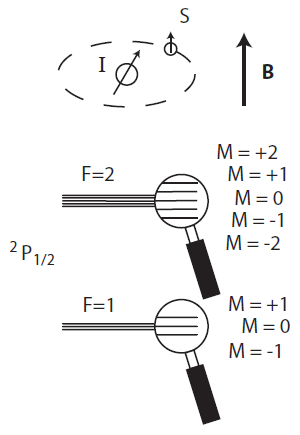
\includegraphics[width = \linewidth]{pictures/Zeeman.png}}
        \begin{subfigure}[t]{0.38\linewidth}
            \centering
            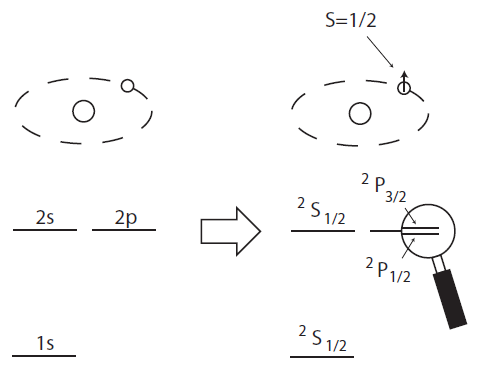
\includegraphics[width = \linewidth]{pictures/Feinstruktur.png}
            \caption{Elektronische Energieniveaus und Feinstruktur von $\ce{^{87}Rb}$.}
            \label{fig:Feinstruktur}
        \end{subfigure}
        \hfill
        \begin{subfigure}[t]{0.26\linewidth}
            \centering
            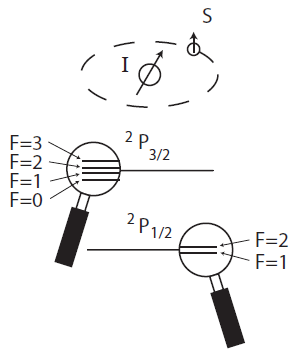
\includegraphics[width = \linewidth]{pictures/Hyperfeinstruktur.png}
            \caption{Hyperfeinstruktur von $\ce{^{87}Rb}$.}
            \label{fig:Hyperfeinstruktur}
        \end{subfigure}
        \hfill
        \begin{subfigure}[t]{0.26\linewidth}
            \centering
            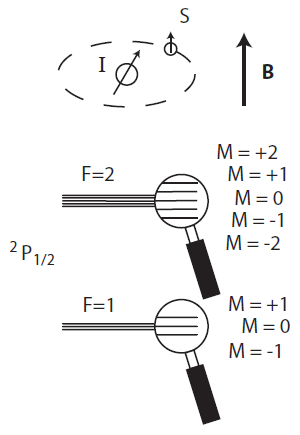
\includegraphics[width = \linewidth]{pictures/Zeeman.png}
            \caption{Zeeman-Aufspaltung der Hyperfeinstruktur von $\ce{^{87}Rb}$.}
            \label{fig:Zeeman}
        \end{subfigure}
        \caption{Hierbei handelt es sich um Darstellungen von Energieniveaus von $\ce{^{87}Rb}$, um diese Konzepte zu verbildlichen. Entnommen aus \cite{httppmawebcaltecheduph77labsoptical-pumpingpdf_optical_nodate}}
    \end{figure}

    \FloatBarrier

    \subsection{Grundlagen zu atomaren Energieniveaus}
        \subsubsection*{Feinstruktur}
            Für diesen Versuch werden Alkalimetalle benutzt, da diese eine ähnliche Struktur wie ein Wasserstoffatom aufweisen.
            Das heißt, dass in allen folgenden Betrachtungen nur das eine Valenzelektron berücksichtigt werden muss.\\
            Bei den hier verwendeten Alkalimetallen handelt es sich um die beiden natürlich vorkommenden Isotope $\ce{^{85}Rb}$ und $\ce{^{87}Rb}$. Im Weiteren beziehen sich alle Formeln und Abbildungen auf diese quasi-ein-Elektron-Atome.

            Der Grundzustand von Alkaliatomen besitzt einen Drehimpuls von $\vec{L} = \vec{0}$ und wird mit 1s bezeichnet.
            Dabei bezieht sich die Zahl auf die Hauptquantenzahl $n = 1$ und der Buchstabe auf die Nebenquantenzahl $l = 0$.

            Die Feinstruktur, wie sie in \autoref{fig:Feinstruktur} zu sehen ist, ergibt sich, wenn der Spin des Elektrons $s = \frac{1}{2}$ in die Betrachtung miteinfließt.
            Die beiden Drehimpulse $\vec{L}$ und $\vec{S}$ koppeln, da der Kern aus Sicht des Elektrons ein Magnetfeld ausstrahlt, und führen zu einer Aufspaltung der Energieniveaus.\\
            Dadurch wird eine andere Notation praktischer, die den Gesamtdrehimpuls $\vec{J} = \vec{L} + \vec{S}$ benutzt:
            \begin{equation*}
                ^{2S+1}L_J
            \end{equation*}
            Hierbei steht das $L$ für den Bahndrehimpuls (S, P, D usw.), das $S = \frac{1}{2}$ für den Spin und das $J$ für den Gesamtdrehimpuls.
            Der Gesamtdrehimpuls wird nach den Regeln der Drehimpulsaddition in dem Bereich von $|L - S|$ bis $|L + S|$ berechnet.
            Die Hauptquantenzahl $n$ wird nicht mehr explizit dazugeschrieben.

            Im dem Fall von $\ce{^{87}Rb}$ wird
            \begin{itemize}
                \item der Grundzustand mit $^2\text{S}_{\nicefrac{1}{2}}$,
                \item der erste angeregte Zustand mit $^2\text{P}_{\nicefrac{1}{2}}$,
                \item der zweite angeregte Zustand mit $^2\text{P}_{\nicefrac{3}{2}}$
            \end{itemize}
            bezeichnet.

        \subsubsection*{Hyperfeinstruktur}
            Hier wird zusätzlich auch der Kernspin $\vec{J}$ betrachtet. Dieser koppelt nach dem gleichen Prinzip der $L$-$S$-Kopplung an $\vec{J}$, sodass sich der Gesamtdrehimpuls $\vec{F} = \vec{J} + \vec{I}$ ergibt und sich die Energieniveaus aufspalten.
            Die Werte für $F$ gehen hier auch analog in Einser-Schritten von $|J - I|$ bis $|J + I|$.

            Für $\ce{^{87}Rb}$ ergibt sich mit dem Kernspin von $I = \frac{3}{2}$ eine Aufspaltung die in \autoref{fig:Hyperfeinstruktur} zu sehen ist. Das $^2\text{S}_{\nicefrac{1}{2}}$-Niveau wird genauso aufgespalten, wie das $^2\text{P}_{\nicefrac{1}{2}}$-Niveau, da beide Energieniveaus $J = \frac{1}{2}$ besitzen.

        \subsubsection*{Zeeman}
            Bei einem angelegten Magnetfeld $\vec{B}$ werden die Energieniveaus noch weiter aufgespalten.
            Wird der Kernspin vernachlässigt ist die Wechselwirkungsenergie mit dem Magnetfeld gegeben als,
            \begin{equation*}
                \Delta E_{\text{ZM,}J} = g_J \mu_0 m_J B
            \end{equation*}
            wobei $\mu_0$ das Bohrsche Magneton ist und $g_J$ der Lande-Faktor mit
            \begin{equation}
                g_J = \frac{3J(J+1) + S(S+1) - L(L+1)}{2J(J+1)}
                \label{eqn:g_J}
            \end{equation}
            ist. Der Faktor kommt daher, dass bei der Bildung des magnetischen Moments des Spins der "anomale Spin-g-Faktor" $g_S = 2$ dazukommt.

            Das gesamte magnetische Moment des Gesamtdrehimpulses $\vec{J}$ ist:
            \begin{equation*}
                \vec{\mu}_J = \vec{\mu}_L + \vec{\mu}_S = \frac{q}{2m_{\text{e}}} \left(g_L \vec{L} + g_S \vec{S}\right)
            \end{equation*}
            $q$ ist dabei die Ladung und $m_\text{e}$ die Masse des Elektrons. $g_L = 1$ wird einfach nur zur Symmetrie dazugeschrieben. Da $g_L \neq g_S$ sind $\vec{J}$ und $\vec{\mu_J}$ nicht parallel und weil sich die senkrechte Komponente über die Zeit herausmittelt, wird die parallele Komponente $\mu_{\text{eff}}$ benutzt, um $g_J$ herzuleiten:
            \begin{equation*}
                \mu_{\text{eff}} = \frac{(\vec{\mu} \cdot \vec{J})}{\vec{J}^2} \vec{J} = g_J \frac{q}{2m_{\text{e}}} \vec{J}
            \end{equation*}
            Nach $g_J$ umgeformt ergibt sich \eqref{eqn:g_J} mit den Eigenwerten $\vec{J}^2 = \hbar^2 J (J+1)$, $\vec{L}^2 = \hbar^2 L (L+1)$ und $\vec{S}^2 = \hbar^2 S (S+1)$.

            Wird der Kernspin auch berücksichtigt ist die Wechselwirkungsenergie mit dem Magnetfeld gegeben als,
            \begin{equation*}
                \Delta E_{\text{ZM,}F} = g_F \mu_0 m_F B
            \end{equation*}
            mit dem Lande-Faktor:
            \begin{equation*}
                g_F = g_J \frac{F(F+1) + J(F+1) - I(I+1)}{2F(F+1)}
            \end{equation*}

    \subsection{Auswahlregeln und Emission}
        Das Licht welches Elektronen in höhere Energieniveaus angeregt bringt gewisse Auswahlregeln an die Übergänge mit sich. Diese Auswahlregeln gelten auch für die Emmission.\\
        Im folgenden bedeutet das $\Delta = $ (Endzustand) - (Anfangszustand):
        \begin{itemize}
            \item $\Delta F = \pm 1$
            \item $\Delta m_F = 0 \qquad$ linear pol. Licht
            \item $\Delta m_F = +1 \qquad$ rechtspol. Licht / $\sigma^- -$Licht
            \item $\Delta m_F = -1 \qquad$ linkspol. Licht / $\sigma^+ -$Licht
        \end{itemize}
        Nach einer gewissen Zeit relaxieren die Elektronen durch Zufall wieder in ihren Grundzustand. Die dabei freiwerdende Strahlung wird gleichmäßig in alle Raumwinkel abgegeben. Dieser Prozess wird spontane Emission genannt.

        Stimulierte Emission passiert, wenn durch Bestrahlung eines äußeren EM-Feldes ein Photon mit genau der Energiedifferenz zwischen dem jetzigen Zustand und einem energetisch niedrigerem Zustand auf das Atom trifft. Dies führt dazu, dass das Atom in den niedrigeren Zustand wechselt und zusätzlich zum einfallenden Photon ein ihm kohärentes Photon abstrahlt. (D.h. Richtung und Frequenz sind gleich.)\\
        Der Übergang muss jedoch die oben genannten Auswahlregeln beachten.

    \subsection{Optisches Pumpen}        
        Da die Energieniveaus bei der Aufspaltung verbunden mit der Hyperfeinstruktur und dem Zeeman-Effekt eine Energiediffernz mit $\Delta E << k_B T$ aufweisen, sind die Wahrscheinlichkeiten dafür, dass sich ein Valenzelektron im Grundzustand (1s, $^2\text{S}_{\nicefrac{1}{2}}$) in einem Zustand mit beliebigem $F$ und $m_F$ aufhält, gleichverteilt. Wird dieses Elektron jedoch angeregt, kann es nur in, durch die Auswahlregeln diktierten, Zustände übergehen.

        In diesem Versuch wird rechts-zirkular polarisiertes Licht auf ein Gas aus Alkaliatomen gestrahlt, wobei ein dazu paralleles Magnetfeld angelegt wird. \autoref{fig:OptischesPumpen} stellt beispielsweise das Konzept des Optischen Pumpens an Wasserstoff dar. Das rechts-zirkular polarisierte Licht bewirkt $\Delta m_F = +1$ und natürlich auch $\Delta F = \pm 1$ weswegen ein Elektron, welches schon den höchsten $m_F$ -Zustand in $^2\text{S}_{\nicefrac{1}{2}}$ besetzt, keinen noch höheren $m_F$ -Zustand in $^2\text{P}_{\nicefrac{1}{2}}$ erreichen bzw. nicht angeregt werden kann.\\
        Befindet sich das Elektron in den anderen $m_F$ -Zustand in $^2\text{S}_{\nicefrac{1}{2}}$ so wird es beim Anregen in einen um $\Delta m_F = +1$ höheren Zustand gebracht.

        Beim Relaxieren fallen die Elektronen unter spontaner Emission in einen Zustand mit $\Delta m_F = 0, \pm 1$. D.h., dass sie im Durchschnitt bei jedem Relaxationsprozess einen Zustand mit $\Delta m_F = 0$ einnehmen.

        Wiederholt sich der Prozess der Anregung und Emission werden die Elektronen nach und nach in den höchsten $m_F$ -Zustand in $^2\text{S}_{\nicefrac{1}{2}}$ gebracht. Für Rubidium funktioniert das Optische Pumpen analog, nur die Anzahl der Energieniveaus wäre größer und der gepumpte Zustand wäre nicht $m_F = +1$, sondern $m_F = +2$.
    
        \begin{figure}
            \centering
            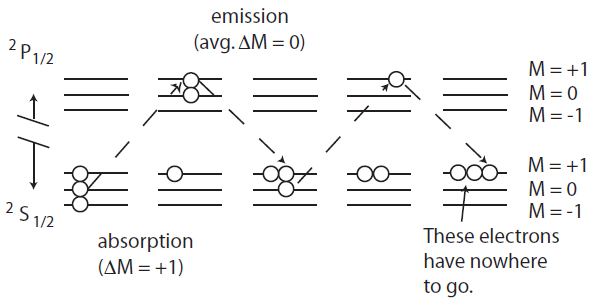
\includegraphics[width = 0.6\textwidth]{pictures/OptischesPumpen.png}
            \caption{Das ist die Darstellung der Methode des Optischen Pumpen zwischen den ($F=1$)-Zuständen in Wasserstoff, wobei das Gas mit rechts-zirkular polarisiertem Licht bestrahlt wird.}
            \label{fig:OptischesPumpen}
        \end{figure}

        \FloatBarrier

    \subsection{Abhängigkeit der Transmission}
        Bei nicht eingeschaltetem Magnetfeld $B = 0$ kann es keine Zeeman-Aufspaltung der Zustände geben, das Licht der Spektrallampe wird vom Rubidiumgas absorbiert und durch spontane Emission wieder abgegeben. Es kommt wenig Licht an der Photodiode an, weswegen es einen Dip im Diagramm gibt, wo die Transmission gegen das angelegte Magnetfeld aufgetragen wird.

        Wird das Magnetfeld erhöht, passiert die Zeeman-Aufspaltung und das Optische Pumpen setzt ein. Dieses führt zu einer Anhäufung der Elektronen im höchsten $m_F$ -Zustand, welche dann kein Licht mehr absorbieren und die Transmission steigt bis auf einen gewissen Wert.

        Wird ein RF-Feld angelegt mit $E_{\text{RF}}$, erreicht das steigende Magnetfeld irgendwann den Punkt, an dem $\Delta E_{\text{ZM},F} = E_{\text{RF}}$ gilt. Ist diese Bedingung erfüllt, wird damit stimulierte Emission erzeugt und die optisch gepumpten Elektronen im höchsten $m_F$ -Zustand können auf tiefere Energieniveaus relaxieren. Somit gibt es mehr Elektronen, die in der Lage sind das Licht der Spektrallampe zu absorbieren und die Transmission hat einen Dip.

        Aus der Bedingung $2 \cdot g_F \mu_B B = E_{\text{RF}}$ kann nach Umstellen der Kernspin leicht bestimmt werden.